\subsubsection{The big picture}

The following picture gives an overview of the different semantics. Elements printed in black are formally defined and proved in the present work, while the gray square on the left shows the proofs and propositions in Launchbury’s original work \cite{launchbury}.

\begin{center}
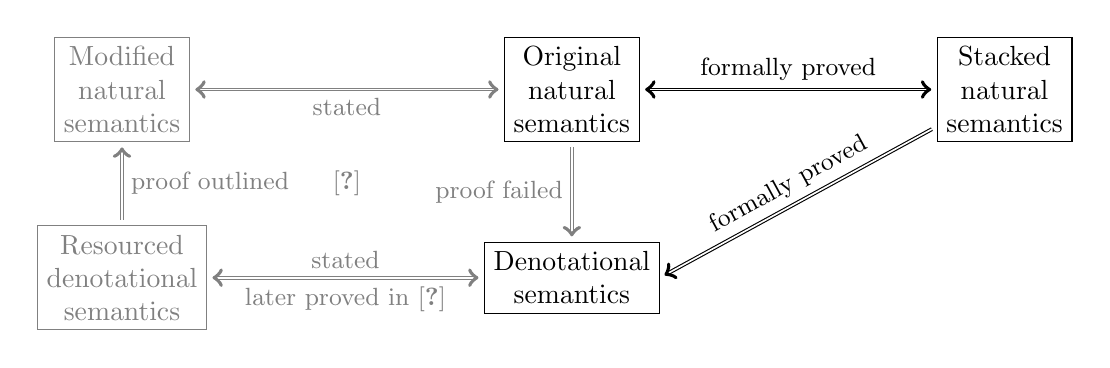
\begin{tikzpicture}[every node/.style={align=center}]
\matrix (m) [row sep=3em, column sep=10em] 
{ \node[draw,gray] (mn) {Modified\\natural\\semantics}; & \node[draw] (on) {Original\\natural\\semantics}; & \node[draw] (sn) {Stacked\\natural\\semantics}; \\
  \node[draw,gray] (rd) {Resourced\\denotational\\semantics}; & \node[draw] (jd) {Denotational\\semantics}; &
  %\node[draw] (ud) {Denotational\\semantics\\with update};
  \\
};

\small
\draw[gray,<->,double, shorten <=.5ex, shorten >= .5ex]  (on) -- (mn) node[midway,below] {stated};
\draw[gray,->,double, shorten <=.5ex, shorten >= .5ex]  (rd) -- (mn) node[midway,right] {proof outlined};
\draw[gray,<->,double, shorten <=.5ex, shorten >= .5ex]  (rd) -- (jd) node[midway,above] {stated} 
                                                            node[midway,below] {later proved in \cite{functionspaces}}; \draw[gray,->,double, shorten <=.5ex, shorten >= .5ex] (on) -- (jd) node[midway,left] {proof failed};
\draw[<->,double, shorten <=.5ex, shorten >= .5ex]  (on) -- (sn) node[midway,above] {formally proved};
\draw[->,double, shorten <=.5ex, shorten >= .5ex] (sn) -- (jd.east) node[sloped,midway,above] {formally proved};
%\draw[->,double, shorten <=.5ex, shorten >= .5ex] (on) -- (ud) node[sloped,midway,above] {Proof};
%\draw[<->,double, shorten <=.5ex, shorten >= .5ex]  (jd) -- (ud) node[midway,below] {formally proved};
\node[gray] at (barycentric cs:on=1,mn=1,rd=1,jd=1) {\cite{launchbury}};
\end{tikzpicture}
\end{center}
